% !TEX root = ../TV-Denoising.tex

\section{The extended support}\label{sec:extended}

Let $f\in \LDD$, with $J(f)<+\infty$, such that $\partial J(f)\neq \emptyset$, or equivalently that~\eqref{eq-constr-dual} has a solution (source condition). 
Let $\voo$ be the corresponding minimal norm certificate and let us define the extended support as
\begin{equation*}
  \ext(Df) \eqdef \overline{\bigcup\enscond{  \supp Dg}{\voo\in \partial J(g)}}.
\end{equation*}
As we shall see in Section~\ref{sec:stab_extended_spt}, the extended support governs the location of $\Supp (D\ulaw)$ for $(\la,w)$ in some low noise regime.


\subsection{Properties of the extended support}
A first remark in view of Proposition~\ref{prop:prelim-suppdf} is that we may rewrite the extended support as 
\begin{equation}\label{eq:extdfperim}
  \ext(Df) = \overline{\bigcup\enscond{\partial^*E}{\abs{E}<+\infty \qandq  \pm\int_E \voo =P(E)}}.
\end{equation}
The inclusion of $\ext(Df)$ in the right hand-side of the above equation is clear by Proposition~\ref{prop:prelim-suppdf}. The converse inclusion is obtained by considering, for any $E$ in the right hand-side, the function $g=\bun{E}$, so as to have $g\in L^2$ and $\voo\in \partial J(g)$ (since $\overline{\partial^*E}=\supp(Dg)$).

From the above equalities, we see that \textit{all the properties of Section~\ref{sec:proplev} (lower and upper boundedness of the perimeter, uniform boundedness\ldots) hold for the elements of the right hand-side whose union determines the extended support.}





The rest of the section is devoted to examples of extended supports, in the case of indicator function of convex calibrable sets or more general convex sets.

\subsection{Convex Calibrable sets}\label{sec:ext_calib}

Let $C\subset \RR^2$ be a bounded convex calibrable set. We wish to describe the extended support of $f=\bun{C}$. This may be done by looking at a vector field $z$ with divergence  $\voo$ (see Section~\ref{sec:calibrable}), which is more informative, or by the following approach.

By Proposition~\ref{prop:mincertcalib}, we know that the minimal norm certificate associated to $f=\bun{C}$ is $\voo=h_C\bun{C}$, where $h_C=\frac{P(C)}{\abs{C}}$. By~\eqref{eq:extdfperim}, we are thus led to solve
\begin{align}
  \label{eq:extendedcalibmoins}   \inf_{\substack{E\subset\RR^2\\\abs{E}<+\infty}} P(E)-h_C \abs{E\cap C},\\
  \label{eq:extendedcalibplus}  \mbox{and } \inf_{\substack{E\subset\RR^2\\\abs{E}<+\infty}} P(E)+h_C \abs{E\cap C}.
\end{align}
Problem~\eqref{eq:extendedcalibplus} is trivial and its only solution is $\emptyset$, so that we only focus on~\eqref{eq:extendedcalibmoins}. By Proposition~\ref{prop:prelimcalibminimal}, we see that $E=C$ is a minimizer. 
Moreover, since $C$ is convex, for all $E$ with finite perimeter $P(C\cap E)\leq P(E)$ with strict inequality whenever $\abs{E\setminus C}>0$. As a result, any other solution must satisfy $E\subseteq C$. But with this condition, either $E=\emptyset$ or $E$ is a solution to the Cheeger problem
\begin{equation*}
  \min_{E\subseteq C} \frac{P(E)}{\abs{E}}.
\end{equation*}
The uniqueness of the solution to the Cheeger problem inside any convex set is proved in~\cite{giusti78,alteruniq09}, and we already know that $C$ is optimal. As a result, either $E=\emptyset$ or $E=C$, and eventually
\begin{equation*}
  \ext(Df)= \partial C.
\end{equation*}

\subsection{Smooth convex sets}\label{sec:ext_smooth}
Let $C\subset\RR^2$ be a bounded open convex set with $\Cder{1,1}$ boundary. We describe the extended support of $f=\bun{C}$ by considering the minimal norm certificate $\voo$ defined in~\eqref{eq:convexvc}.
We need to study the solutions of 
\begin{align}
  \label{eq:extendedcvxmoins}   \inf_{\substack{E\subset\RR^2\\\abs{E}<+\infty}} P(E)-\int_E \voo,\\
  \label{eq:extendedcvxplus}  \mbox{and } \inf_{\substack{E\subset\RR^2\\\abs{E}<+\infty}} P(E)+\int_E \voo.
\end{align}
Since $\voo\geq 0$, we see that the only solution to~\eqref{eq:extendedcvxplus} is $\emptyset$.
As for~\eqref{eq:extendedcvxmoins}, the same convexity argument as above shows that any solution must be included in $C$. 

Now let $r\in [\rho_0, R]$, where $1/\rho_0\geq \ess\sup_{x\in\partial C}\kappa(x)$ and $C_r$ be the opening of $C$ with radius $r$ as defined  in Section~\ref{sec:MNC_convex}. Denoting by $\nu_{C_r}$ the outer unit normal to $\partial C_r$, we have
\begin{equation*}
  P(C_r)=\int_{\partial C_r}z_0\cdot \nu_{C_r}\d \Hh^1 =\int_{C_r}\divx z_0 =\int_{C_r}\voo,
\end{equation*}
hence $C_r$ is a solution to~\eqref{eq:extendedcvxmoins} and  $\ext(Df) \supseteq \overline{\bigcup\enscond{\partial C_r}{\rho_0\leq r\leq R}}$.

Let us prove that there is no solution $E$ such that the reduced boundary $\partial^*E$ intersects $C_R$. 
By Remark~\ref{rem:countunion}, the solutions to~\eqref{eq:extendedcvxmoins} are stable by intersection. If a solution $E$ is such that $E\cap C_R\neq \emptyset$, then $P(E\cap C_R)=\int_{E\cap C_R}\voo = h_{C_R}\abs{E\cap C_R}$ where $h_{C_R}=\frac{P(C_R)}{\abs{C_R}}$ and $E\cap C_R$ is a solution to the Cheeger problem
\begin{equation*}
  \min_{F\subseteq C_R} \frac{P(F)}{\abs{F}}. 
\end{equation*}
By uniqueness of the Cheeger set of $C_R$, we obtain that $E\cap C_R=C_R$.
Eventually, we have proved 
\begin{equation}
  \ext(Df) =\overline{\bigcup\enscond{\partial C_r}{\rho_0\leq r\leq R}}.
\end{equation}


\begin{figure}[H]
\begin{center}
\begin{tabular}{c@{\hspace{15pt}}c@{\hspace{35pt}}c@{\hspace{15pt}}c}
        
\begin{tikzpicture}[scale=2]

\fill[black] (.5,.5) circle(5mm);
\end{tikzpicture}
&
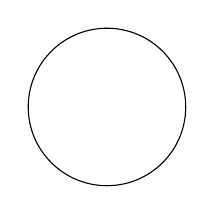
\begin{tikzpicture}[scale=2]

\draw[black] (.5,.5) circle(5mm);
\end{tikzpicture}&

\begin{tikzpicture}[scale=2]
        \fill  [rounded corners=5pt, fill=black] (0,0)--(1,0)--(1,1)--(0,1)--cycle;
       % \draw (.265,.265) circle(.265);
        
        \end{tikzpicture}&

\begin{tikzpicture}[scale=2]
        \fill  [rounded corners=5pt, fill=black] (0,0)--(1,0)--(1,1)--(0,1)--cycle;
        \fill  [rounded corners=15pt, fill=white] (0,0)--(1,0)--(1,1)--(0,1)--cycle;
       % \draw (.265,.265) circle(.265);
        
        \end{tikzpicture}
\\
$\bun{A}$ & $\ext(D\bun{A})$ &$\bun{B}$ & $\ext(D\bun{B})$
\end{tabular}
\end{center}

\caption{Examples of the extended support for two indicator functions. }

\end{figure}

